%% AstroCLIP schematic — contrastive alignment of galaxy images and SFHs
%% Compile with: pdflatex astroclip_schematic.tex
\documentclass[tikz, border=14pt]{standalone}
\usepackage{tikz}
\usepackage{amsmath}
\usetikzlibrary{arrows.meta, calc, backgrounds, decorations.pathreplacing, fit, positioning}
\usepackage{amssymb}
\usepackage{graphicx}

%% ── colour palette ───────────────────────────────────────────────────────────
\colorlet{imgcol}{blue!60!black}
\colorlet{sfhcol}{orange!80!black}
\colorlet{embcol}{teal!60!black}
\colorlet{poscol}{violet!70!black}      %% positive-pair connector
\colorlet{boxbg}{gray!11}

\tikzset{
  %% thumbnail frames
  imgbox/.style = {draw=imgcol!50, fill=boxbg, rounded corners=3pt,
                   minimum size=1.65cm, line width=0.75pt, inner sep=0pt},
  sfhbox/.style = {draw=sfhcol!50, fill=boxbg, rounded corners=3pt,
                   minimum size=1.65cm, line width=0.75pt, inner sep=0pt},
  %% encoder blocks  (#1 = border/fill colour)
  encbox/.style = {draw=#1, fill=#1!7, rounded corners=7pt,
                   minimum width=2.0cm, minimum height=5.6cm,
                   line width=1.1pt, align=center, font=\small},
  %% embedding vector bars  (#1 = colour)
  embvec/.style = {draw=#1!75, fill=#1!22, rounded corners=2pt,
                   minimum width=0.42cm, minimum height=1.30cm, line width=0.65pt},
  %% arrows
  myarr/.style  = {-{Stealth[length=5pt,width=4pt]}, line width=0.9pt,
                   draw=#1, shorten >=2pt, shorten <=2pt},
}

\begin{document}
\begin{tikzpicture}[font=\small]

%% ── y positions of the three galaxy examples ─────────────────────────────────
\def\ya{4.40}   % galaxy 1 (top)
\def\yb{2.30}   % galaxy 2 (middle)
\def\yc{0.20}   % galaxy 3 (bottom)

%% ═══════════════════════════════════════════════════════════════════════════
%% LEFT COLUMN — galaxy image thumbnails
%% ═══════════════════════════════════════════════════════════════════════════
%% Real JWST COSMOS-Web stamps (colour composite: R=ch2, G=ch1, B=ch0)
%% galaxy 1 = rising SFH, galaxy 2 = declining SFH, galaxy 3 = bursty SFH
\node[imgbox] (im1) at (0, \ya)
  {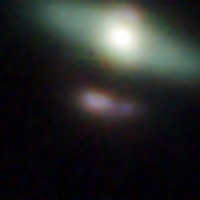
\includegraphics[width=1.65cm,height=1.65cm]{gal_rising.png}};
\node[imgbox] (im2) at (0, \yb)
  {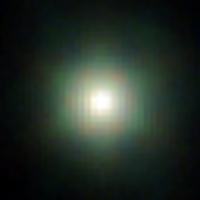
\includegraphics[width=1.65cm,height=1.65cm]{gal_declining.png}};
\node[imgbox] (im3) at (0, \yc)
  {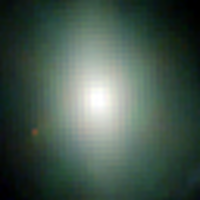
\includegraphics[width=1.65cm,height=1.65cm]{gal_bursty.png}};

%% small colour dot: row identifier
\fill[red!70!black]    ([xshift=-3pt,yshift=-3pt]im1.north east) circle (2.5pt);
\fill[green!60!black]  ([xshift=-3pt,yshift=-3pt]im2.north east) circle (2.5pt);
\fill[blue!60!black]   ([xshift=-3pt,yshift=-3pt]im3.north east) circle (2.5pt);

\node[above=5pt of im1, font=\small\bfseries, color=imgcol] {Galaxy images};

%% brace labelling N pairs on the left
\draw[decorate, decoration={brace, amplitude=6pt, mirror},
      gray!50, line width=0.6pt]
  ([xshift=-10pt]im3.south west) -- ([xshift=-10pt]im1.north west);
\node[font=\scriptsize, color=gray!65, rotate=90, anchor=south]
  at ([xshift=-18pt]im2.west) {$N$ training pairs};

%% ═══════════════════════════════════════════════════════════════════════════
%% RIGHT COLUMN — SFH thumbnails
%% ═══════════════════════════════════════════════════════════════════════════
\node[sfhbox] (sh1) at (11.6, \ya) {};
\node[sfhbox] (sh2) at (11.6, \yb) {};
\node[sfhbox] (sh3) at (11.6, \yc) {};

%% --- SFH 1 : rising (bar heights increase old→recent, i.e. left→right) ---
\begin{scope}
  \clip (sh1.south west) rectangle (sh1.north east);
  \fill[sfhcol!72] ([xshift= 3pt,yshift=5pt]sh1.south west) rectangle ++( 9pt, 9pt);
  \fill[sfhcol!72] ([xshift=14pt,yshift=5pt]sh1.south west) rectangle ++( 9pt,17pt);
  \fill[sfhcol!72] ([xshift=25pt,yshift=5pt]sh1.south west) rectangle ++( 9pt,28pt);
  \fill[sfhcol!72] ([xshift=36pt,yshift=5pt]sh1.south west) rectangle ++( 9pt,40pt);
\end{scope}
\draw[gray!45, line width=0.35pt]
  ([xshift=2pt,yshift=4pt]sh1.south west) -- ([xshift=-2pt,yshift=4pt]sh1.south east);
\node[font=\tiny, color=gray!60, anchor=north west, inner sep=0pt]
  at ([xshift=2pt,yshift=2pt]sh1.south west) {\tiny$0$};
\node[font=\tiny, color=gray!60, anchor=north east, inner sep=0pt]
  at ([xshift=-2pt,yshift=2pt]sh1.south east) {\tiny$t_H$};

%% --- SFH 2 : declining ---
\begin{scope}
  \clip (sh2.south west) rectangle (sh2.north east);
  \fill[sfhcol!72] ([xshift= 3pt,yshift=5pt]sh2.south west) rectangle ++( 9pt,42pt);
  \fill[sfhcol!72] ([xshift=14pt,yshift=5pt]sh2.south west) rectangle ++( 9pt,28pt);
  \fill[sfhcol!72] ([xshift=25pt,yshift=5pt]sh2.south west) rectangle ++( 9pt,14pt);
  \fill[sfhcol!72] ([xshift=36pt,yshift=5pt]sh2.south west) rectangle ++( 9pt, 5pt);
\end{scope}
\draw[gray!45, line width=0.35pt]
  ([xshift=2pt,yshift=4pt]sh2.south west) -- ([xshift=-2pt,yshift=4pt]sh2.south east);
\node[font=\tiny, color=gray!60, anchor=north west, inner sep=0pt]
  at ([xshift=2pt,yshift=2pt]sh2.south west) {\tiny$0$};
\node[font=\tiny, color=gray!60, anchor=north east, inner sep=0pt]
  at ([xshift=-2pt,yshift=2pt]sh2.south east) {\tiny$t_H$};

%% --- SFH 3 : bursty ---
\begin{scope}
  \clip (sh3.south west) rectangle (sh3.north east);
  \fill[sfhcol!72] ([xshift= 3pt,yshift=5pt]sh3.south west) rectangle ++( 9pt,24pt);
  \fill[sfhcol!72] ([xshift=14pt,yshift=5pt]sh3.south west) rectangle ++( 9pt, 8pt);
  \fill[sfhcol!72] ([xshift=25pt,yshift=5pt]sh3.south west) rectangle ++( 9pt,36pt);
  \fill[sfhcol!72] ([xshift=36pt,yshift=5pt]sh3.south west) rectangle ++( 9pt,14pt);
\end{scope}
\draw[gray!45, line width=0.35pt]
  ([xshift=2pt,yshift=4pt]sh3.south west) -- ([xshift=-2pt,yshift=4pt]sh3.south east);
\node[font=\tiny, color=gray!60, anchor=north west, inner sep=0pt]
  at ([xshift=2pt,yshift=2pt]sh3.south west) {\tiny$0$};
\node[font=\tiny, color=gray!60, anchor=north east, inner sep=0pt]
  at ([xshift=-2pt,yshift=2pt]sh3.south east) {\tiny$t_H$};

%% row-identifier triangles on SFH thumbnails (triangles = SFH modality)
\fill[red!70!black]
  ([xshift=-4pt,yshift=-5pt]sh1.north east) +(-3pt,-2pt) -- +(3pt,-2pt) -- +(0pt,3.5pt) -- cycle;
\fill[green!60!black]
  ([xshift=-4pt,yshift=-5pt]sh2.north east) +(-3pt,-2pt) -- +(3pt,-2pt) -- +(0pt,3.5pt) -- cycle;
\fill[blue!60!black]
  ([xshift=-4pt,yshift=-5pt]sh3.north east) +(-3pt,-2pt) -- +(3pt,-2pt) -- +(0pt,3.5pt) -- cycle;

\node[above=5pt of sh1, font=\small\bfseries, color=sfhcol]
  {Star formation histories};

%% brace on the right
\draw[decorate, decoration={brace, amplitude=6pt},
      gray!50, line width=0.6pt]
  ([xshift=10pt]sh3.south east) -- ([xshift=10pt]sh1.north east);
\node[font=\scriptsize, color=gray!65, rotate=-90, anchor=south]
  at ([xshift=18pt]sh2.east) {$N$ training pairs};

%% ═══════════════════════════════════════════════════════════════════════════
%% ENCODERS
%% ═══════════════════════════════════════════════════════════════════════════
\node[encbox=imgcol] (imgenc) at (3.4, 2.3)
  {\bfseries Image\\\bfseries encoder\\[6pt]$f_\theta(\cdot)$};

\node[encbox=sfhcol] (sfhenc) at (8.2, 2.3)
  {\bfseries SFH\\\bfseries encoder\\[6pt]$g_\phi(\cdot)$};

%% ═══════════════════════════════════════════════════════════════════════════
%% EMBEDDING VECTORS
%% ═══════════════════════════════════════════════════════════════════════════
\node[embvec=imgcol] (ie1) at (5.3, \ya) {};
\node[embvec=imgcol] (ie2) at (5.3, \yb) {};
\node[embvec=imgcol] (ie3) at (5.3, \yc) {};

\node[embvec=sfhcol] (se1) at (6.3, \ya) {};
\node[embvec=sfhcol] (se2) at (6.3, \yb) {};
\node[embvec=sfhcol] (se3) at (6.3, \yc) {};

\node[below=3pt of ie3, font=\footnotesize\itshape, color=imgcol]
  {$\mathbf{z}^{\text{img}}$};
\node[below=3pt of se3, font=\footnotesize\itshape, color=sfhcol]
  {$\mathbf{z}^{\text{SFH}}$};

%% ═══════════════════════════════════════════════════════════════════════════
%% FLOW ARROWS
%% ═══════════════════════════════════════════════════════════════════════════
\foreach \i in {1,2,3}{
  %% image → encoder → embedding
  \draw[myarr=imgcol] (im\i.east)            -- (imgenc.west  |- im\i);
  \draw[myarr=imgcol] (imgenc.east |- ie\i)  -- (ie\i.west);
  %% SFH → encoder → embedding
  \draw[myarr=sfhcol] (sh\i.west)            -- (sfhenc.east  |- sh\i);
  \draw[myarr=sfhcol] (sfhenc.west |- se\i)  -- (se\i.east);
}

%% ═══════════════════════════════════════════════════════════════════════════
%% POSITIVE-PAIR CONNECTORS  (same galaxy → same row)
%% ═══════════════════════════════════════════════════════════════════════════
\foreach \i/\col in {1/red!70!black, 2/green!60!black, 3/blue!60!black}{
  \draw[\col, dashed, line width=1.1pt, shorten >=1pt, shorten <=1pt]
    (ie\i.east) -- (se\i.west);
}

%% ═══════════════════════════════════════════════════════════════════════════
%% CONTRASTIVE LOSS BOX  (well below the architecture, centred)
%% ═══════════════════════════════════════════════════════════════════════════
\node[draw=embcol!50, fill=white, rounded corners=5pt,
      align=center, font=\small, text=embcol,
      inner sep=7pt, minimum width=3.2cm] (loss) at (5.8, -2.0)
  {\bfseries Contrastive loss (InfoNCE)\\[4pt]
   $\mathcal{L} = -\frac{1}{N}\sum_{i}
     \log\frac{
       \exp(\mathbf{z}_i^{\text{img}}\cdot\mathbf{z}_i^{\text{SFH}}/\tau)}{
       \sum_{j}\exp(\mathbf{z}_i^{\text{img}}\cdot\mathbf{z}_j^{\text{SFH}}/\tau)}$};

%% faint arrows from the bottom embedding row down to the loss box
\draw[-{Stealth[length=4pt]}, embcol!40, line width=0.7pt]
  (ie3.south) -- ([xshift=-12pt]loss.north);
\draw[-{Stealth[length=4pt]}, embcol!40, line width=0.7pt]
  (se3.south) -- ([xshift= 12pt]loss.north);

%% ═══════════════════════════════════════════════════════════════════════════
%% SHARED EMBEDDING SPACE
%% ═══════════════════════════════════════════════════════════════════════════
\node[draw=embcol!50, fill=white, rounded corners=7pt,
      align=center, font=\small\bfseries, text=embcol,
      minimum width=5.0cm, minimum height=2.2cm,
      inner sep=8pt] (emb) at (5.8, -4.5)
  {Shared embedding space\\[45pt]};

%% arrow from loss to shared space
\draw[-{Stealth[length=5pt,width=4pt]}, embcol!60, line width=1.0pt]
  (loss.south) -- (emb.north);

%% ── 6-symbol UMAP: circle = image embedding, triangle = SFH embedding ───
%% Matched pairs share a colour; each pair is spatially close in latent space.
%% emb box centre ≈ (5.8, -4.5); usable x ∈ [4.0, 7.6], y ∈ [-5.0, -4.0]
\begin{scope}
  \clip (emb.south west) rectangle (emb.north east);
  %% Red pair  (galaxy 1)
  \fill[red!65!black]   (4.30,-4.50) circle (3.0pt);                          % image
  \fill[red!65!black]   (4.60,-4.35) +(-3pt,-2pt) -- +(3pt,-2pt) -- +(0,3.5pt) -- cycle; % SFH
  %% Green pair  (galaxy 2)
  \fill[green!55!black] (5.70,-4.42) circle (3.0pt);                          % image
  \fill[green!55!black] (6.05,-4.58) +(-3pt,-2pt) -- +(3pt,-2pt) -- +(0,3.5pt) -- cycle; % SFH
  %% Blue pair  (galaxy 3)
  \fill[blue!60!black]  (7.10,-4.50) circle (3.0pt);                          % image
  \fill[blue!60!black]  (7.45,-4.35) +(-3pt,-2pt) -- +(3pt,-2pt) -- +(0,3.5pt) -- cycle; % SFH
\end{scope}
%% tiny legend
\node[font=\tiny, text=gray!70, anchor=south west, inner sep=0pt]
  at ([xshift=4pt,yshift=4pt]emb.south west)
  {$\circ$ image \quad $\triangle$ SFH};

\end{tikzpicture}
\end{document}
